\section*{Progress on Simulating function values and inferring $B_a, B_b, B_c$}

\emph{Doesn't work yet.}  Last week, I directly simulated values of $a_i, b_i, c_i$ for patient with covariate $x_i$, assuming no noise in the model ($\phi^a=\phi^b=\phi^c=0$) and was able to infer $B_a, B_b, B_c$, as they were the linear coefficients in \emph{independent} generalized linear models (independent given the data, which in that case was $a_i, b_i, c_i$).

However this week, the data is no longer $a_i, b_i, c_i$, but actual function values for a patient at particular times, $g_i^*(t; a_i, b_i, c_i)$.  I fix $B_a, B_b, B_c$.  Simulation is done with no noise - equivalent to setting $\phi^a=\phi^b=\phi^c=\phi^{noise}=0$.  Start with a cohort of patients - choose covariates for each patient.  For each patient, I picked a few time points, and added function values at those times as data.   Inference was a lot more difficult here, because now, $B_a, B_b, B_c$ are correlated given the data, which is no longer the $a_i, b_i, c_i$.

\subsection*{Debugging approach}
\begin{itemize}
\item Make $g_i(t;s_i, a_i, b_i, c_i)$ more simple.  Tried:
  \begin{enumerate}
    \item $g_i(t;s_i, a_i, b_i, c_i) = a_i$.  Then, $B_b$ and $B_c$ are independent of the data and come from the prior.  Don't have to worry about correlation of $B_a$ with other parameters.  This works.
    \item $g_i(t;s_i, a_i, b_i, c_i) = a_i + b_i*t$.  $B_c$ is independent of the data.  Posterior for $B_a$ and $B_b$ are correlated, but inference still worked.
    \item $g_i(t;s_i, a_i, b_i, c_i) = s_i[(1-a_i) - b_i(1-a_i)(e^{-t})]$.  This did not work.  Plots to follow.
  \end{enumerate}
\item Forcing noise parameters to be close to 0 by making $\lambda_a, \lambda_b, \lambda_c, \lambda_{noise}$ very high.
\item Trying Metropolis Hastings vs Adaptive Metropolis Hastings didn't help in case 3.
\end{itemize}

\subsection*{Diagnostic plots for error case}
Simulation was done using $g_i$ as in item 3 above.  Selected 1 dimensional covariate for 15 patients.  Set $B_a=-1.0, B_b=1.0, B_c=1.0$.  I start the MCMC from the MLE parameters.
\begin{itemize}
\item Figure 1: Set all parameters to maximum likelihood values.  Then, vary $B_a, B_b, B_c$ one at a time, holding other parameters fixed to see if likelihood surface is flat there.
\item Figure 2: The simulated datapoints.  The actual times I chose to 'measure' the function values at are denoted by the dots.  Purpose was to see if changing the covariate $x_i$ affected the corresponding curves.
\item Figures 3 and 4: Trace of parameters that vary in the chain.
\item Figure 5: Histogram of $B_a,B_b,B_c$.
\item Figure 6: The curves of the patients, plotted using the mean posterior value for $B_a, B_b, B_c$.  Purpose was to see whether, despite the coefficients being different, if the curves looked similar.
\end{itemize}

\begin{figure}
\begin{center}
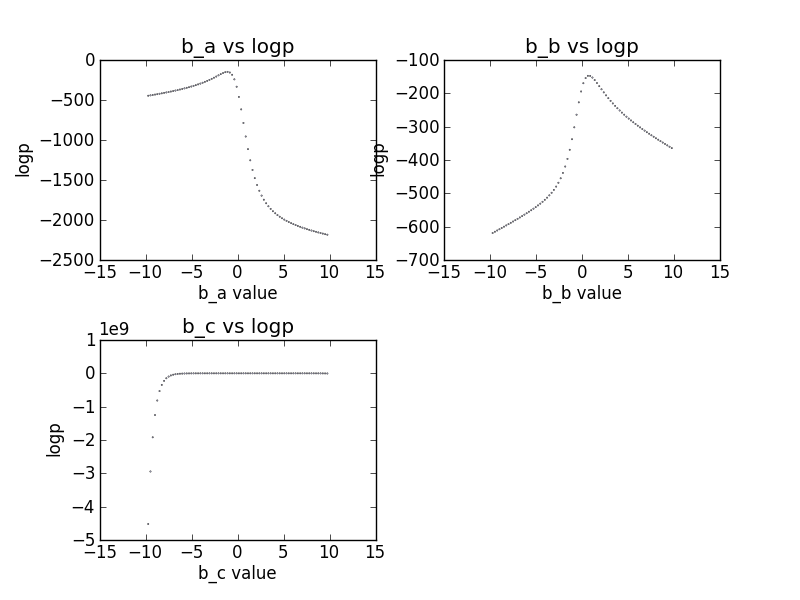
\includegraphics[width=5in, height=4in]{/Users/glareprotector/prostate_git/glare/tex_files/sections/simulate_data_points_infer_Bs/files/likelihood_vs_Bs.png}
\caption{Likelihood surface vs $B_a, B_b, B_c$ at MLE}
\end{center}
\end{figure}

\begin{figure}
\begin{center}
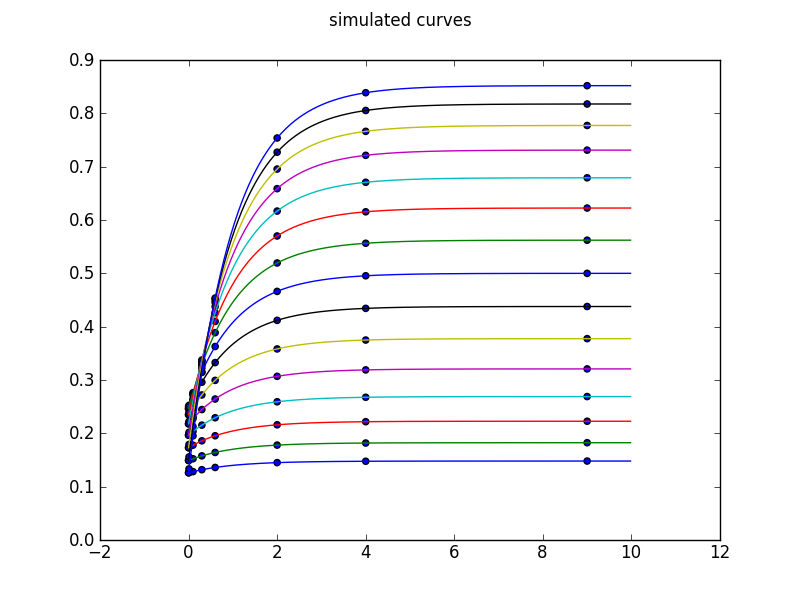
\includegraphics[width=5in, height=4in]{/Users/glareprotector/prostate_git/glare/tex_files/sections/simulate_data_points_infer_Bs/files/simulated_curves.png}
\caption{Simulated Curves of the Cohort}
\end{center}
\end{figure}

\begin{figure}
\begin{center}
\includegraphics[width=5in, height=4in]{/Users/glareprotector/prostate_git/glare/tex_files/sections/simulate_data_points_infer_Bs/files/Bs_trace2.png}
\caption{Trace of $B_a, B_b, B_c$}
\end{center}
\end{figure}

\begin{figure}
\begin{center}
\includegraphics[width=5in, height=4in]{/Users/glareprotector/prostate_git/glare/tex_files/sections/simulate_data_points_infer_Bs/files/rhos_trace.png}
\caption{Trace of $\phi$'s}
\end{center}
\end{figure}

\begin{figure}
\begin{center}
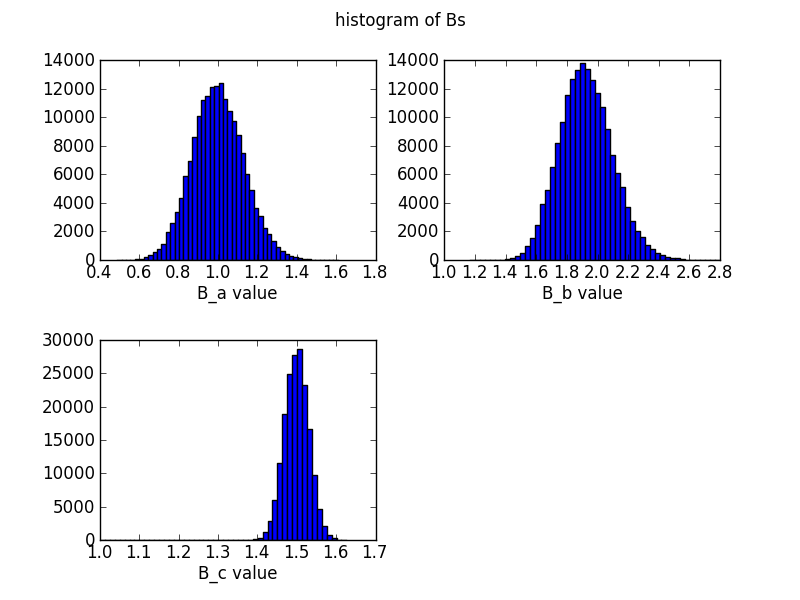
\includegraphics[width=5in, height=4in]{/Users/glareprotector/prostate_git/glare/tex_files/sections/simulate_data_points_infer_Bs/files/Bs_histogram.png}
\caption{Histogram of $B_a, B_b, B_c$}
\end{center}
\end{figure}

\begin{figure}
\begin{center}
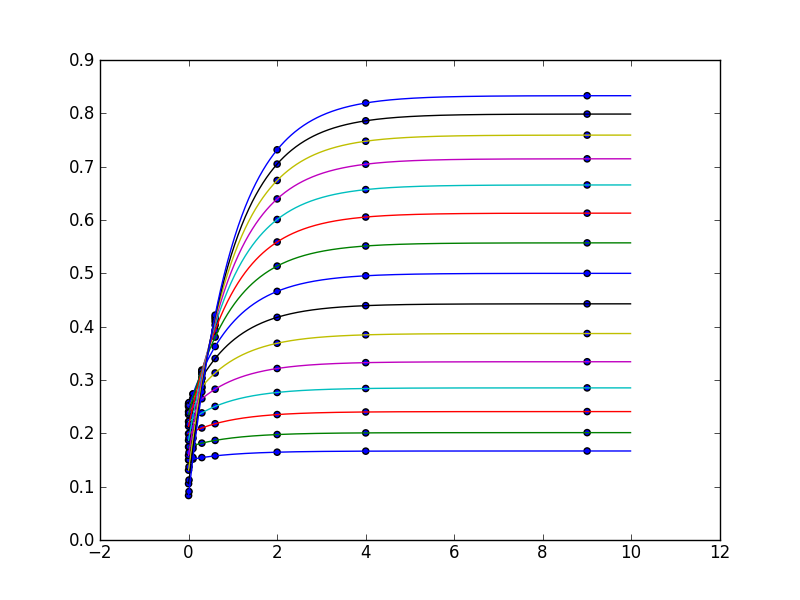
\includegraphics[width=5in, height=4in]{/Users/glareprotector/prostate_git/glare/tex_files/sections/simulate_data_points_infer_Bs/files/posterior_curves.png}
\caption{Posterior Curves of the Cohort}
\end{center}
\end{figure}